\section{Photon Normalization}\label{sec:analysis.gflux}
In the calculation of the differential cross-section, Sec.~\ref{sec:results}, accuracy of the total number of photons incident on the target will determine the accuracy of the cross-section measurement. The procedure for determining the total number of photons in CLAS has already been established in~\cite{clas.gflux}. This procedure was performed for the \g12 data set and is discussed further in~\cite{clas.g12.note}. In this analysis, only events which were in the ``good'' scalar interval were considered. A ``good'' scalar interval relates to data recorded when the photon flux was recorded in ``live-time''. ``Live-time'' is the time that the data acquisition was ready to record events in conjunction with CLAS. For this analysis the photon flux, gflux, was binned in increments of 25~MeV and can be seen in Fig.~\ref{fig:gflux}. The 25 MeV binning was chosen to compare past experiments differential cross-sections with this analysis.

It should be noted that beam energies with values $3.025 \pm 25$~MeV, $3.075 \pm25$~MeV, $3.125 \pm25$~MeV and $3.525 \pm25$~MeV bins are excluded from the analysis due to flux calculation problems that arose from dead scintillators in the tagger. 

\begin{figure}[h!]\begin{center}
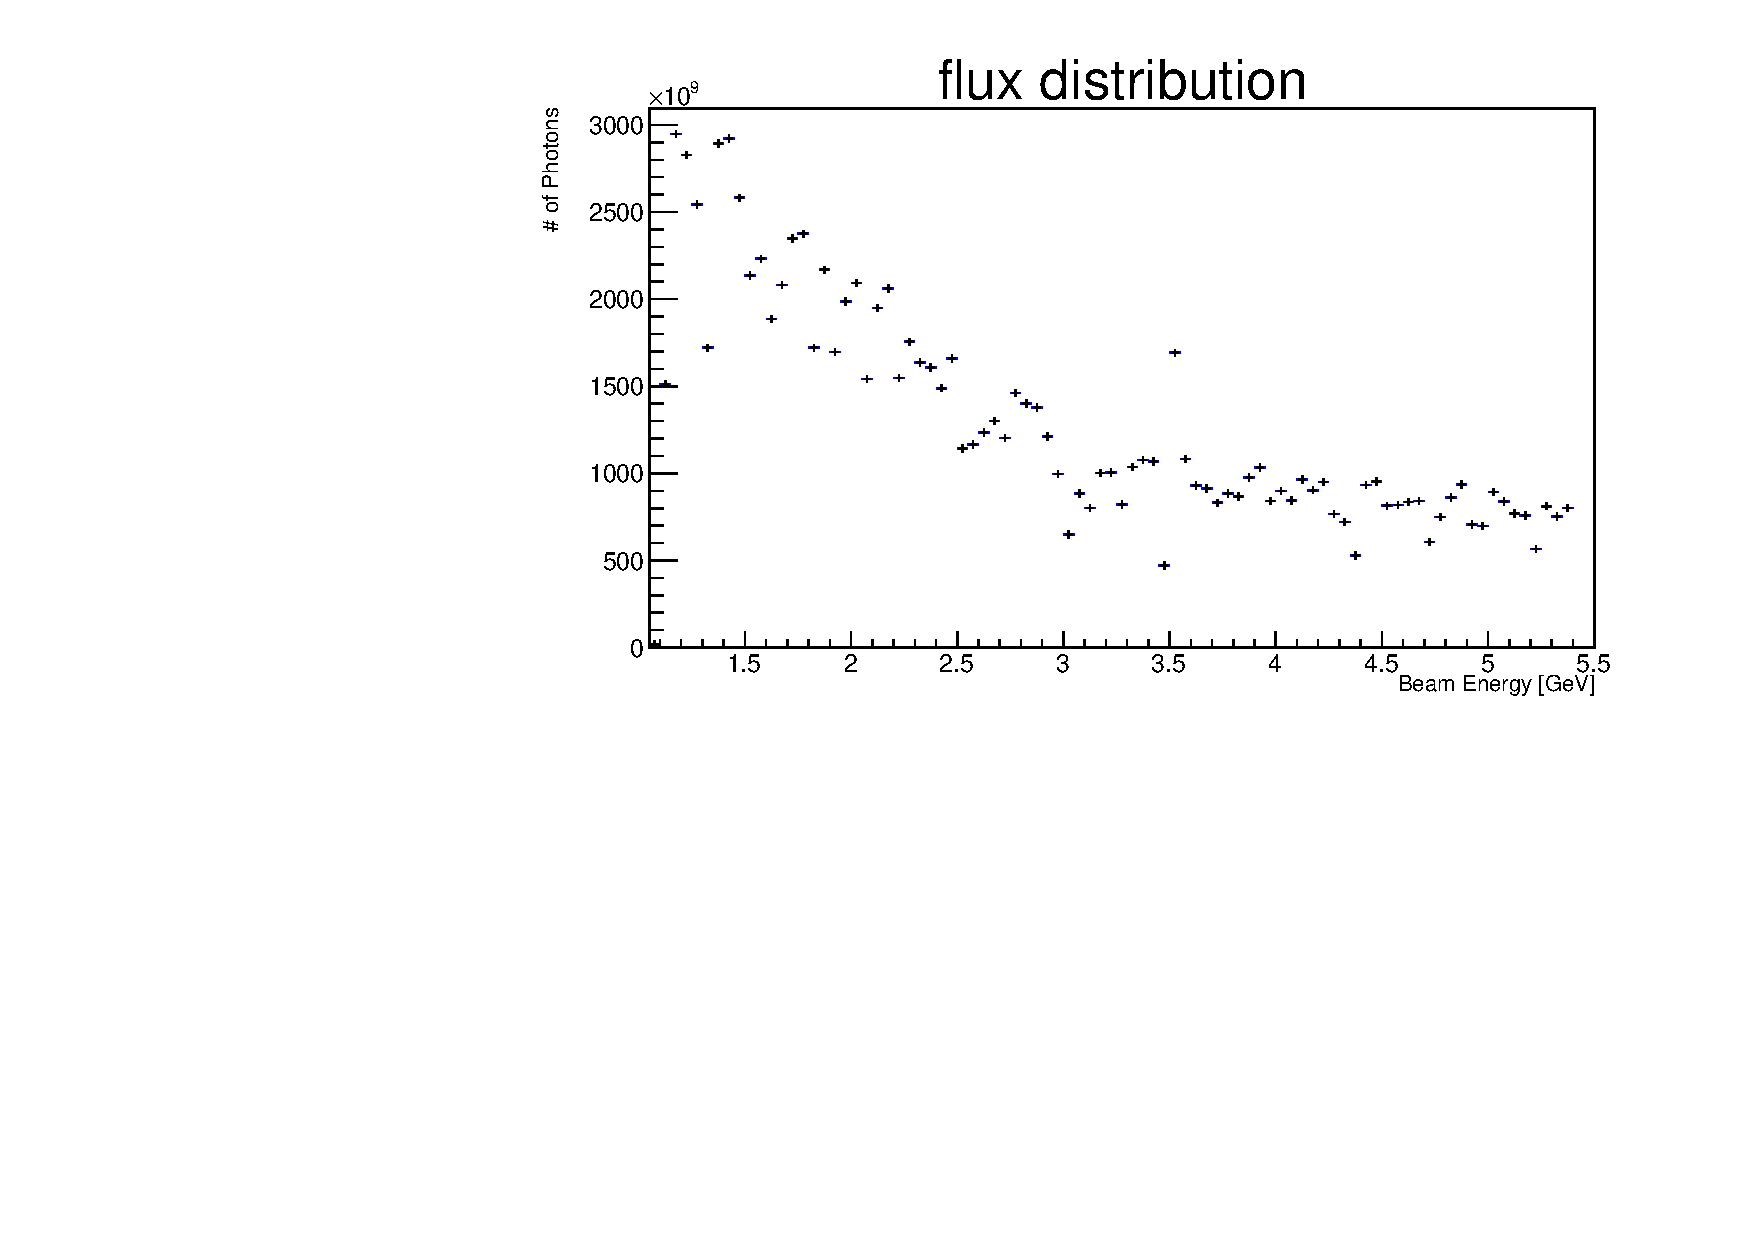
\includegraphics[width=\figwidth,height= 0.75 \hfigheight]{\figures/analysis/GFLUX/Analysis_GFlux_II.pdf}
\caption[Photon flux for analysis]{\label{fig:gflux}Photon flux for analysis}
\end{center}\end{figure}
\FloatBarrier

%\subsection{Gflux}